\documentclass[journal]{IEEEtran}
\usepackage[a5paper, margin:10mm, onecolumn]{geometry}
\usepackage{amsmath,amssymb,amsfonts,amsthm}
\usepackage{mathtools}
\usepackage{gvv-book}
\usepackage{gvv}
\usepackage{hyperref}

\begin{document}

\title{12.163}
\author{Puni Aditya - EE25BTECH11046}
\maketitle

\textbf{Question:}

The geometric transformation specified by
\begin{align*}
    \myvec{X' & Y' & 1} = \myvec{X & Y & 1} \myvec{0.5 & 0 & 0 \\ 0 & 0.25 & 0 \\ 1 & 2 & 1}
\end{align*}
in a 2D CAD system represents
\begin{enumerate}
    \item Scaling and Translation
    \item Scaling and Rotation
    \item Rotation and Translation
    \item Rotation
\end{enumerate}

\textbf{Solution:}

A 2D affine transformation is of the form $\vec{x}'^\top = \vec{x}^\top\vec{T}$, where the transformation matrix is
\begin{align*}
    \vec{T} = \myvec{
        \vec{A} & \vec{0} \\
        \vec{t}^\top & 1
    }
\end{align*}
The given transformation matrix is:
\begin{align}
    \vec{T} = \myvec{0.5 & 0 & 0 \\ 0 & 0.25 & 0 \\ 1 & 2 & 1}
\end{align}
From this, we identify the linear transformation matrix $\vec{A}$ and the translation vector $\vec{t}$.
\begin{align}
    \vec{A} = \myvec{0.5 & 0 \\ 0 & 0.25}, \quad \vec{t} = \myvec{1 \\ 2}
\end{align}
Since $\vec{A}$ is a diagonal matrix and not a multiple of the identity, it represents a non-uniform scaling. Since $\vec{t} \neq \vec{0}$, there is a translation.

A pure rotation requires the linear part $\vec{A}$ to be an orthogonal matrix, where $\vec{A}\vec{A}^\top = \vec{I}$. We check this condition:
\begin{align}
    \vec{A}\vec{A}^\top = \myvec{0.5 & 0 \\ 0 & 0.25}\myvec{0.5 & 0 \\ 0 & 0.25} = \myvec{0.25 & 0 \\ 0 & 0.0625} \neq \vec{I}
\end{align}
Since $\vec{A}$ is not orthogonal, the transformation is not a rotation.

\textbf{Example:} Applying the transformation to the point $\myvec{1 \\ 1}$. In homogeneous coordinates,
\begin{align}
    \vec{x}'^\top &= \myvec{1 & 1 & 1} \myvec{0.5 & 0 & 0 \\ 0 & 0.25 & 0 \\ 1 & 2 & 1} \\
    &= \myvec{1(0.5)+1(0)+1(1) & 1(0)+1(0.25)+1(2) & 1(0)+1(0)+1(1)} \\
    &= \myvec{1.5 & 2.25 & 1}
\end{align}
The point $\myvec{1 \\ 1}$ is transformed to $\myvec{1.5 \\ 2.25}$, demonstrating both scaling and translation.

The correct option is \textbf{1) Scaling and Translation}.

\begin{figure}[h!]
    \centering
    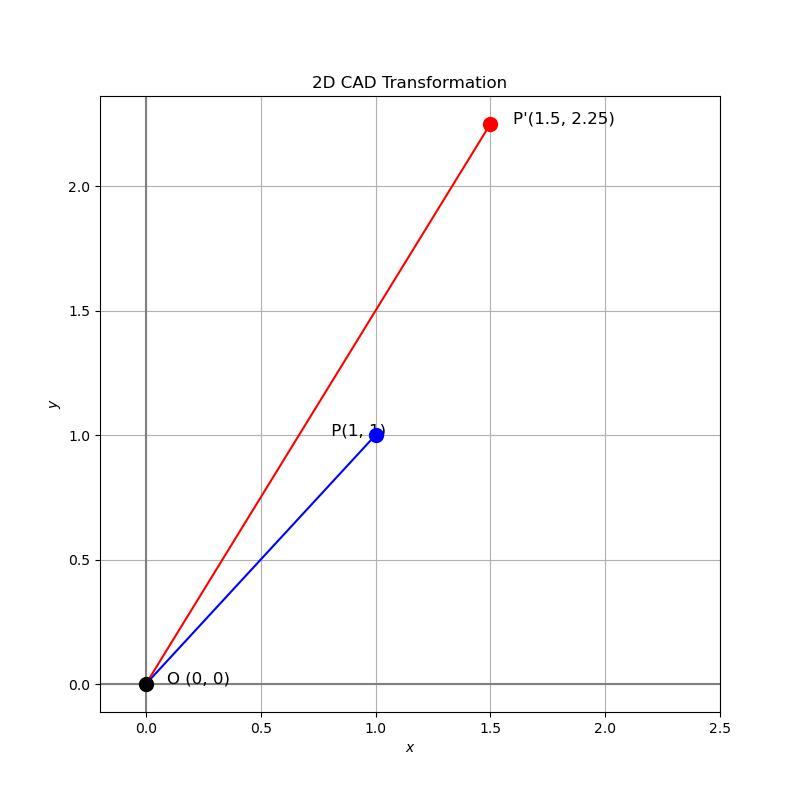
\includegraphics[width=\columnwidth]{figs/plot_p.jpg}
    \caption*{Plot}
    \label{fig:fig}
\end{figure}

\end{document}
